\section{Prestudy and research}
As mentioned in the project introduction, the quality of the final solution would rely on our ability to research and understand the medical industry. While both of the customers had experience with software development in this industry, their field of knowledge were mainly limited to the area of professional medical imaging. Based on this, the customer requested information about how other parts of the IT infrastructure worked, with a special focus on how to get patient data in and out of an electronic medical record. 

\subsection{Method}
Because of the need for extensive research, this chapter is not limited to "prestudies". Research spanned the whole project and had to be done in parallel with the development. The research method have revolved around getting a hold of and communicating with different key persons in the Norwegian industry, listed in Appendix \ref{contacts}. At the beginning of the project, the two biggest questions we set out to answer were: 

\begin{itemize}
\item How are the existing systems compiled?
\item What kind of systems will the application be dependent on?
\end{itemize}

As discovered, uploading directly to an "EMR" was not necessary the solution. In this chapter, we will present the findings of how the Norwegian industry and environment work. This implies that some details about systems will differ from hospital to hospital. In order to avoid confusion we will start by presenting terminology and technology in a historical context, commenting the extent of our research along the way.

\subsection{The history of EMRs}
\label{sec:history}
In the 1960s and '70s, early efforts were done to utilize computers in order to store and manage medical records overseas. Aerospace manufacturer Lockheed Martin developed one such system, a \emph{clinical information system} as they were called \cite{ehrDevelopment}. Already in the 1980s, one started to see the benefits of industry-wide standards. This led to the first initiative to standardize this information, and nonprofit standards developing organizations (SDOs) started to form. They would facilitate the widespread use and organization of electronic medical information.
\noindent
One of these initiative takers was Health Level 7 (HL7). Since 1987 they have became the most widely recognized SDO in the industry of medical information technology. They develop electronic standards to ensure that the different departmental systems can exchange clinical data in a meaningful way. This is essential because modern hospital information systems (HIS) are often composed of components made by many different vendors. Since the beginning, HL7 have released numerous messaging standards. With a coverage of 95\% in the US healthcare organizations, HL7v2 is by far the most used messaging protocol for clinical data today \cite{hl7numbers}. A discussion on HL7 and other standards follows later in this chapter.

\subsection{Medical imaging}
The installation of a platform to organize medical images, like the one Lockheed Martin developed for the EMRs in the mid 60s, saw the light of day in 1982. This platform was called a Picture Archiving and Communication System (PACS). With new image management systems emerging, the radiographic community saw the need for a standardized format these systems could utilize. In 1985 The American College of Radiology (ACR) and National Electrical Manufacturers Association (NEMA) released their first standard. It was called ACR/NEMA 300, but would later be recognized as the Digital Imaging and Communications standard (DICOM). 
Like HL7 is the industry standard for text based clinical information, DICOM is the industry standard for handling, storing and transmitting data in medical imaging today \cite{dicom_standard}. As the name suggest this standard include both a file format e.g. a way of structuring the data, as well as a protocol to transport it over. 

This was the first format we set out to explore. As this is the most used format and protocol for medical imaging, we thought a PACS would be the place to upload images to. Based on that information, we spent a good amount of time learning the details in this standard in order to upload images.

%%%%%%%%%%%%%%%%%%%% NY SUBSECTION %%%%%%%%%%%%%%%%%%%%


\subsection{Understanding the environment}
\label{sec:understandingEnvironment}
In this section we will first give an explanation of the central interoperability issues existing in today's systems, before we explain how a typical hospital IT environment is structured.

As mentioned, a modern hospital information system (HIS) can be compiled of multiple, both dependent and independent software solutions from different vendors. Below we will discuss the connection between selected solutions.
\noindent
The common denominator between the components that constitute the HIS, is the messaging protocols standardized by the SDOs. As mentioned earlier, this is the gap HL7 set out to fill. Already in 1989 HL7 introduced their HL7v2 standard. An example of a HL7v2 message can be seen in Figure \ref{fig:hl7sample}. Here, fields are separated by pipes, hence the nickname \emph{Pipehat}:

\begin{figure}[H]
\centering
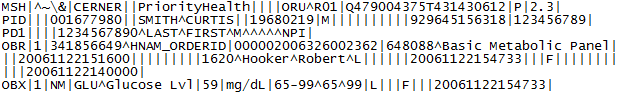
\includegraphics[scale=0.8]{img/hl7sample.png}
\caption{HL7v2 sample message}
\label{fig:hl7sample}
\end{figure}

\noindent
As HL7v2.x was the most used messaging protocol by far, the group initially thought our solution depended on our understanding of this standard in order to get patient data from a hospital information system.

To date there has been released 9 versions of HL7v2, represented generically as HL7v2.x. Although the v2.x standards are backward compatible, it does not have the strongest foundation; it was built in a "bottom-up" approach that has addressed individual needs. There is no underlying reference model and the first version was released only two years after the HL7 organization was founded. With 25 years of infrequent additions to the standard it is loosely defined and suffers - as others have suggested \cite{evolution:hl7} and \cite{rel:openehr} - from too much optionality. Because of this, situations where two systems supporting HL7v2 don't necessarily interoperate occur, because they implement different parts of the standard. This again has led to additional initiatives like the Integrating Healthcare Enterprise (IHE) \cite{ihe} which is focusing its work into specifying integration \emph{profiles} based on clinical domains. In other words, they are trying to standardize different parts of an existing standard. This is also adversely, as hospitals end up using different profiles that don't work together.
Typically, a hospital IT infrastructure is built around a centralized patient administration system (PAS). Surrounding it is several departmental systems, such as those for laboratory, radiology etc. A system for managing medical records is usually closely associated with the PAS, hence the commonly used abbreviation PAS/EMR. These services are made accessible through terminals stationed at individual departments usually running the Windows operating system. As we've learned (Heidi Torstunsen, personal communication, February-April, 2014), the hospitals strive to keep the number of credentials associated to one person to a minimum, and they are often identical across different logins. Despite the central PAS/EMR, departmental systems may also have their own systems for managing information about patients treated there. As Roald Bergstrøm told us, this is the case in the radiology department: Here the PACS gets patient information from a radiology information system (RIS) (meeting, February 28, 2014). Overlapping systems like this is not uncommon in the hospital environment; it has do with the concurrent development of the individual systems. The PACS exchanges textual metadata directly to the EMR in form of a \emph{report}. This happens via HL7 messages, as seen in Figure \ref{fig:theEnvironment} on the next page. This means that some information about a patient's radiology examination can be found in the PAS/EMR. The whole examination with images can be viewed through a web view connecting to the PACS where the images are stored.

\begin{figure}[H]
\centering
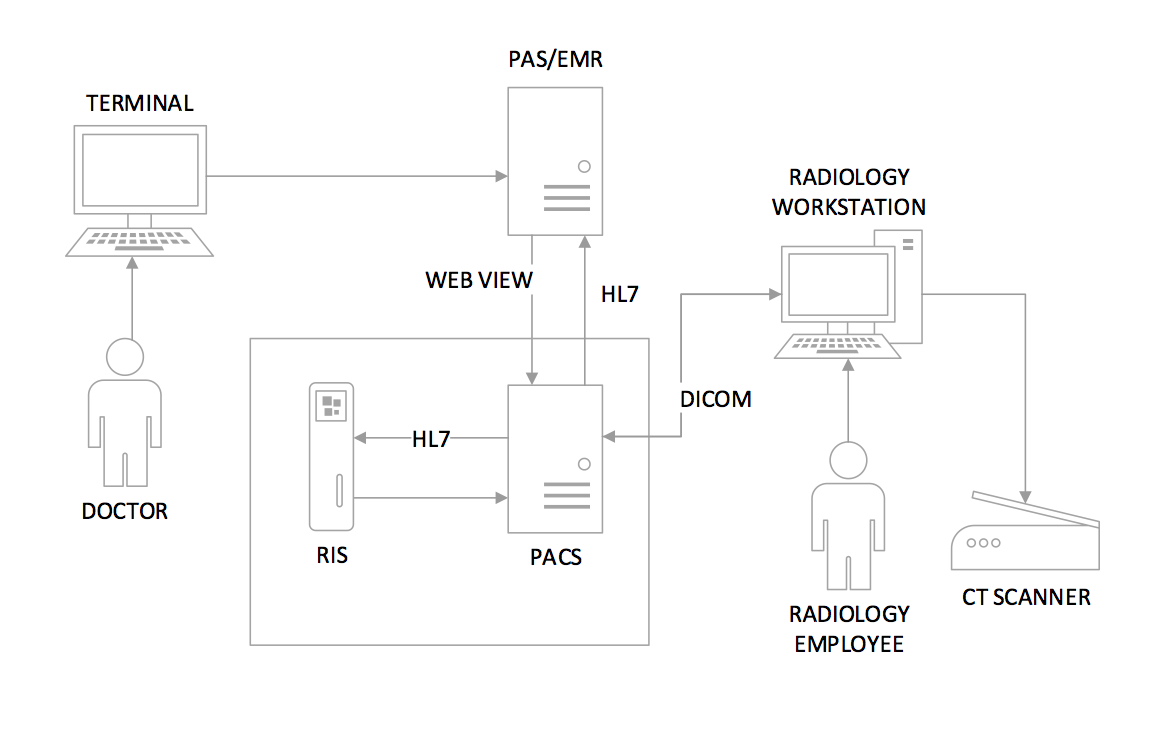
\includegraphics[scale=0.6]{img/env_chart.png}
\caption{A selected portion of the environment}
\label{fig:theEnvironment}
\end{figure}


%%%%%%%%%%%%%%%%%%%% NY SUBSECTION %%%%%%%%%%%%%%%%%%%%

\subsection{Today and the future}
After sprint 4, described in section \ref{sprint4}, it was decided to put some additional effort into researching future solutions and standards. This section will cover the work that is currently being done in the industry in order to solve interoperability issues in today's systems.

\subsubsection{HL7v3 and openEHR}
Despite it's popularity, even HL7 acknowledged that v2.x had some legacy issues. To avoid the burden of the these issues, they decided it would not be backward compatible. Starting from scratch they first defined a reference information model (RIM) \cite{hl7RIM}, which they based the third messaging standard, HL7v3 on. These messages have a more familiar XML syntax.

Through conversations with Roald Bergstrøm from KITH \cite{KITH}, we were introduced to what the future holds for hospital IT infrastructure and electronic medical records. He told us that in Australia, a group of researches spent more than 15 years of research to develop and test an open, detailed and comprehensive interoperable health information computing platform. Its called openEHR \cite{openEHR}, and is based on a two-level modeling approach, known as the ‘archetype methodology’. Archetypes is a way of structuring data, where you clearly define clinical information models. This makes it possible to separate a information system's data model from the clinical one. Several SDOs believe this is the future for interoperable data between clinical systems and shared EMRs. Over the last couple of years, the architecture have influenced the development of EHR standards by both CEN (European Committee for Standardization), HL7 and ISO (International Organization for Standardization) \cite{rel:openehr}. In Norway the process of defining, quality assure, approve and share archetypes on a national scale was initiated by the The Western Norway Regional Health Authority \cite{helseVest}, and is currently in progress.

Based on this methodology, HL7 released a standard document structure specifying the structure and semantics of clinical documents. It is called Clinical Document Architecture (CDA) and is based on XML Schemas \cite{hl7CDAR2}. These documents are still thought to be exchanged by the HL7v3 messaging standard. The standard is currently in its second release (CDA R2), and have already been adopted by DIPS (see section \ref{exsol}). Figure \ref{fig:HL7relationship} illustrates the relationship between openEHR, CEN13606 and HL7. For more information, see Ocean Informatics article on the relationship between CEN 13606, HL7, and openEHR\cite{rel_openehr1}.

\begin{figure}[H]
\centering
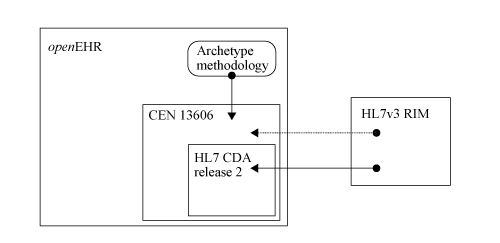
\includegraphics[scale=0.8]{img/relationship.png}
\caption{The relationship between openEHR and HL7\cite{rel_openehr1}}
\label{fig:HL7relationship}
\end{figure}



%%%%%%%%%%%%%%%%%%%% NY SUBSECTION %%%%%%%%%%%%%%%%%%%%


%%THE VSCAN DEVICE
\subsection{The Vscan device and ultrasound}
\label{vscan}
The existing Vscan device is a handheld, pocket-sized visualization tool powered by ultrasound technology. The device was first introduced in 2010, after being developed by GEs Norwegian department GE Vingmed, based in Horten. The device is bundled with a desktop application called Gateway, which allows for importing and organizing images and video. This is done through a docking station that is connected to the computer via an USB cable. The latest version of this software support reporting capabilities by generating PDF (Portable Document Format) reports from an examination. An example report can be found in Appendix \ref{existingGatewayReport}.

The customers intend to improve the original Vscan product. At the first meeting the group were told that GE had reason to believe that all ultrasound specific technology some time in the future would be able to fit inside the probe (Figure \ref{fig:ultraprobe}.b) of the existing product. With these ultrasound probes in mind, the customer envisioned the ability to connect it to a modern smart device (like a smart phone Figure \ref{fig:ultraprobe}.a) over a standard interface like the Universal Serial Bus (USB). These smart devices would then run software applications with a user interface for the scanner.

\begin{figure}[H]
\centering
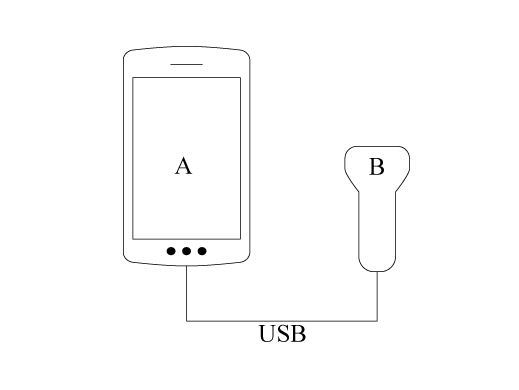
\includegraphics[scale=0.4]{img/ultraprobe.png}
\caption{Smart device (a) with attached ultrasound probe (b)}
\label{fig:ultraprobe}
\end{figure}

\noindent
Although GE developed the first device of this kind, they are not alone on the market: The customer told us that they considered Siemens hand held ultrasound system \cite{ACUSONP10} to be their main competitor. We have found other devices with even greater similarities to the  smart device (with interchangeable probes) solution they now envision \cite{MobiUSSP1}.

The original device and its competitors have introduced the term \textit{pocket ultrasound}. Traditionally ultrasound examinations are performed by professional radiologists or technicians at a radiology department. With pocket ultrasound this workflow changes, and examinations can be conducted in the patient rooms. This improvement in technology opens for more frequent use of ultrasound, and the user group will no longer be restricted to those working in the radiology department. 

The implications of this was \emph{not} obvious to the group at first, as we initially thought the application could rely on PACS for storing ultrasound images. After a detour exploring PACS and DICOM, we realized that uploading data to PACS was impossible, as this was a system exclusively for the radiology department, and unavailable for other medical personnel. Another solution had to be found.


%%%%%%%%%%%%%%%%%%%% NY SUBSECTION %%%%%%%%%%%%%%%%%%%%


\subsection{DIPS}
\label{exsol}
From October this fall, DIPS will be installed at OUS. This combined with their marked share, is the reason we invested time in researching their solutions. 

The same year HL7 started its work, the Norwegian company DIPS (Distribuert Informasjons og Pasiendatasystem i Sykehus) was founded at Nordland Sentralsykehus. They set out to develop \emph{''user friendly software that run on standard hardware in a network''}. Today, they have extended their product line and offer modules for EMR, PAS, Multimedia and Economy to name a few. With more than 70\% coverage of Norwegian hospitals, they are currently Norway's largest vendor of EMR software \cite{DIPS}, with customers in three of the four Regional Health Authorities in Norway \cite{RHF}. They were also the first EMR company in Norway to implement support for many standardized system-to-system protocols, utilizing XML (Extensible Markup Language) and HL7 standards \cite{dips_pioneer}.

Initially, OUS  will get the solution DIPS Classic, which is their old PAS/EMR solution. Through communicating with Konik developers working on integrating this solution in Oslo, the group was given access to an empty DIPS server as described in section \ref{serviceDescription}. 

After communication with Alexander Theodorsen, working at DIPS in Bodø, we got some insight on how their solutions worked, and how it would affect our application. Among other things, he informed us that \emph{Active Directory} was the main user management system used by hospitals in Norway. Based on this, LDAP was chosen as the applications authentication mechanism.


%%%%%%%%%%%%%%%%%%%%%%%%%%%%%%%%%%%%%%%%%%%%%%%%%%%%%%%%%%%

\subsection{Multimedia in hospitals}
\label{multimediaInHospitals}
The storing of images and video on hospital servers are today almost exclusively used by radiologists, but there is a demand for multimedia and smart mobile devices. Researchers think this will become a more central aspect of the daily patient care in the future \cite{indremedisineren}. As mentioned in the introduction of this chapter, a big question for this project resided in where the results of an examination should be stored. As we've covered in the previous sections, we put a good amount of effort into researching systems like PACS and the core EMR in order to store information from our application. Because of the clinical value radiologists add in the PACS, ultrasound images from hand held devices did not belong here. Although DIPS (as an example) support PDF attachments to be uploaded in the actual EMR, these systems are specialized around text-based documents, and do not meet the needs for searching and indexing multimedia. Another issue was pointed out by Heidi Torstunsen (communication, 2014), who told us that current laws and regulations put restrictions on what data that can be stored; only data of a certain clinical value should be stored. Roald Bergstrøm at KITH could confirm this, and said the following:
\newpage
\begin{quote} 
\textit{A national selection has evaluated whether images should be stored in the EMR, and has concluded that the findings of the doctors is the artifact to be considered legally binding. This entails that when ultrasound images are examined and described, this description is applicable and should be saved while the image can be deleted. \\(Translated from Norwegian)}
\end{quote}
\noindent
However, Roald himself consider this to be bad practice and pointed out that X-ray images are saved up to 10 year for further reference. Taking the needs of the customer, as well as feedback we got from stakeholders in the industry into consideration, we decided to not take this into account, as it would end our project. After consulting with the customer we decided to continue researching other possible, future solutions. 

To this date there is no widely recognized system for storing multimedia. The only solutions we could find was \emph{DIPS Multimedia} \cite{dipsmultimedia} and \emph{Seekuence} from Posicom \cite{posicom} which are currently being tested and deployed. These are both pioneers in this market. Both systems takes the form of independent modules ready to be integrated with existing hospital systems like PAS/EMR, and they are built on modern technology supporting a wide array of multimedia formats and protocols. We have yet to figure out how they cope with the issues regarding national rules and regulations in their solutions.

We worked with Bjørn Næss (personal communication, March - May, 2014) to get help implementing a service communicating with DIPS Multimedia. As this solution is still being tested, DIPS did not have any development documentation for us. Bjørn tried to arrange for us to get help from one of their developers, but due to time constraints it did not work out.

%%%%%%%%%%%%%%%%%%%% NY SUBSECTION %%%%%%%%%%%%%%%%%%%%


\subsection{Security}
Security is a topic that can not be avoided when developing software for this industry. In the following section we will give an overview of the most important issues we encountered. After a section on mobile smart devices and memory, we conclude with a simple risk assessment.

\subsubsection{Smart devices}
We believe some consideration regarding possible hardware threats is of interest to the customer. Both Heidi Torstunsen could tell us that devices like this are bought in, and managed at a department level. This means that the department share one or more hand held devices. Due to security reasons, this is likely to stay the same even with the introduction of smart devices. A Bring Your Own Device (BYOD) policy is currently not applicable for clinical devices. From a security point of view, there are a lot of challenges with having a single device shared between multiple unique users. This is outside the scope of this project, but we believe it is important to point out.

To illustrate some of the security concerns regarding mobile smart devices, we have written a short article on possible threats, if the customer should be interested. Based on this research, we concluded to not consider in app memory when assessing the security aspects of our application. Because of this we decided not to include it in the final report. It can be found in Appendix \ref{smartSecurity}.


\subsubsection{Risk assessment}
Through communication with Heidi Torstunsen, responsible for privacy and information security at OUS. Many of the design decisions are a direct result of what she told us and the documents she made accessible. We have designed our application with the concerns from OUS's guidelines in mind \cite{ousDocuments_riskAssesment}. As Heidi stated, the Norwegian rules and regulations on privacy and security are considered strict compared to other Europeean countries. We believe this was a healthy base for our design.

Considering the amount of data stored in the application i.e. the number of patients whose sensitive data is in memory at a given time, the individual customers could do a risk assessment and either acknowledge or reject the risk. The way we see it, this number would typically be low, because only examinations intended to be uploaded (at some point) should enter the application. When uploaded, the examination is deleted. 

The real risk as we see it, is the potential loss of user credentials. Concrete examples on how this could be done is found in Appendix\ref{smartSecurity}. Depending on the national and local policy for access control, this could give the attacker access to information about patients on a department, hospital, regional or national level. 


%%%%%%%%%%%%%%%%%%%% NY SUBSECTION %%%%%%%%%%%%%%%%%%%%

%%STAKEHOLDERS
\subsection{Stakeholders}
When making products for the medical industry, there are a lot of people involved with different interests. In this section, the different stakeholders will be presented.

\subsubsection{Product owner}
The group's contact at Capgemini is Jens Lien. Because he is hired by GE, he is acting on their behalf and therefore considered to be the product owner. He has previous experience with developing software for the medical business, and has a vision for what is to be built. His concerns are: 

\begin{itemize}
\item The application works as intended.
\item The application is finished in the given time period.
\end{itemize}

\subsubsection{Application vendor}
Sigmund Frigstad is a project leader at GE Vingmed, and was in charge of developing the original Vscan device. He is responsible for the Vscan device that the application will be shipped with. His concerns are: 

\begin{itemize}
\item The application runs on the specified platform/hardware.
\item The application communicates with the Vscan application.
\item The application is able to communicate with hospital servers.
\end{itemize}

\subsubsection{End user}
This is the group of users that will use the Vscan device and the application in the hospitals. This group is divided in two; technical users and non-technical users. Non-technical users users are considered to be doctors and other medical personnel certified to perform examinations with a pocket ultrasound device \cite{EFSUMB}. The technical users are considered to be technical staff working at the hospitals. Their concerns are respectively:\\

\textbf{Non-technical user}
\begin{itemize}
\item The application is intuitive to use and eases the work flow of storing ultrasound images.
\item The application is able to save changes before uploading data.
\end{itemize}

\textbf{Technical user}
\begin{itemize}
\item The application can be set up to work with the hospital servers.
\item The need for manual inputting data is minimal when setting up device.
\end{itemize}
\noindent Non-technical users will be referred to as users in the remainder of the report.


\subsubsection{System owner}
This stakeholder can either be the hospital administration itself or an external company delivering systems or services to the hospital. An example of a relationship like this is the Norwegian institution Sykehuspartner \cite{sykehuspartner}. The system owner is responsible for setting requirements for availability, confidentiality, integrity and quality of the systems delivered to, or used on the respective hospital institutions. Their concerns are:

\begin{itemize}
\item That the application meets legal requirements when handling personal information in an hospital environment.
\item That the application meets security requirements set by the specific hospital, district, region or country.
\end{itemize}

\subsubsection{Third-party Developer}
A developer will be needed to customize certain parts of the solution at the individual hospitals. Their concerns are:

\begin{itemize}
\item Good API documentation.
\item All data necessary to upload examination is available.
\end{itemize}


%%%%%%%%%%%%%%%%%%%% NY SUBSECTION %%%%%%%%%%%%%%%%%%%%


%DEV TOOLS AND LIBS
\subsection{Libraries and development tools}

A number of tools and libraries have been used during development of the application. Some of them were required by the customer, but most have been chosen based on the groups preference and experience, and most importantly, because they fit the project needs. A requirement for all the applications used, is that they are free to use and multi platform, as the group got members using both Windows and Mac OSX. It was determined that tools for the following purposes were needed:

\begin{itemize}
\item Development
\item File storing and version control
\item Documentation
\item Communication
\end{itemize}

%DEV TOOLS
\subsubsection{Development tools}
This section contains an overview of the development tools and libraries used in the project.
\paragraph*{Android and Java}
Android is an operating system developed and maintained by Google aimed at smartphones and tablets. The Android platform is released under an open source license and has a large community of developers developing third party libraries and tools. Android is currently the most used mobile operating system in the world \cite{android_pop}. Applications developed for Android are written mainly in Java by using the Android software development kit (SDK), which are highly maintained and very well documented.

The application developed during this project was made for the Android platform. This was a requirement set by the customer and the basis for the project.

\paragraph*{IntelliJ IDEA}
IntelliJ IDEA \cite{intellij} is an IDE (Integrated Development Environment) which supports Android and has integrated support for all major build tools. The build tool support was an important consideration when choosing an IDE, as it may be both hard and time consuming to maintain a large project with many dependencies. The group were recommended to use IntelliJ by the customer representative at Capgemini.

\paragraph*{Genymotion}
When developing for Android, either an emulator or a physical device is needed to simulate the runtime environment for an application. The Android SDK comes bundled with a standard emulator, but it is extremely slow and a hassle to work with. Therefore, the group have been using the Genymotion \cite{genymotion} emulator which is based on Oracle VirtualBox \cite{virtualBox}. Genymotion has increased performance compared to the standard emulator.

\paragraph*{Gradle}
When maintaining a large project, a build tool is very helpful. Gradle \cite{gradle} is a build tool made specifically for Android development. It helps with everything from managing third party libraries and other dependencies, to compiling the project.

%%LIBS
\subsubsection{Libraries}
This section contains an overview of the libraries used in the project. All libraries are free to use, and most are open source.

\paragraph*{SQLite and SQLCipher}
SQLite is an open source, lightweight database management system (DBMS) which is included as a standard in all Android based devices. It is simple to use, universal and got all the functionality needed. Because of its popularity, there are several libraries offering encryption of databases on Android devices running on top of SQLite. The open source project SQLCipher \cite{sqlcipher} was chosen as it offered easy integration with our existing database. SQLCipher offers AES 256 bit encryption.

\paragraph*{Crouton}
Crouton \cite{crouton} is a library which serves as an alternative to the traditional Android \textit{Toast} \cite{toast}. A Toast is a small popup notification that floats on the screen for a given time. The problem with Toast for our use, is that Toasts are context in-sensitive, meaning they do not "belong" to their parent view and will not disappear before they have run their full duration. This could possibly make for some confusing situations for the user, with multiple Toasts floating on the screen. This is where Croutons come in. A Crouton is context sensitive, meaning it will dissapear once its parent view is hidden or removed.

\paragraph*{FlatUI kit and PhotoView}
FlatUI kit \cite{flatui} and PhotoView \cite{photoview} are both libraries used to enhance the UI of the application. The FlatUI kit offers easy integration of attractive UI elements as an alternative to the standard Android look and feel. PhotoView is used to ease the implementation of functionality like zooming and multi-touch gestures in ImageViews.

\paragraph*{UnboundID LDAP}
UnboundID \cite{unboundid} is a SDK for Java, used to provide Lightweight Directory Access Protocol (LDAP) functionality in the application. 

\paragraph*{JCraft JSch}
JSch \cite{jsch} is used in the Android service, and is a library that allows connection to a server through the SSH protocol. 

\paragraph*{iText}
\label{itextlib}
iText \cite{itext} is a library that allows users to both generate and manipulate PDFs. 

\paragraph*{JDBC}
JDBC is used in the Android service, and is a library that allows for communication with a SQL database in Java \cite{JDBC}.
% OBS OBS! Bør skrive om JDBC (brukt i service)

%DOCUMENTATION TOOLS
\subsubsection{Documentation tools}
This section contains an overview of the tools and services used to document code, project process and report writing. See section \ref{project_management_tools} for additional tools used for project management. 

\paragraph*{Git and GitHub}
Git \cite{git} is an open source distributed version control system. Using a version control system allows multiple developers to work on the same code and commit their work to a common repository. Other participants then fetch these changes to their local copy of the repository. Git offers many advanced features. Most importantly, the group has been actively using the branching feature, which allows for different "copies" of the project to be worked on simultaneously. This is useful when implementing features that shouldn't be merged into the main project before they are fully implemented and working as intended. The group were assigned a private repository hosted at GitHub \cite{github} owned by the customer. This way the customer was able to follow the project progress closely.

\paragraph*{Javadoc}
Javadoc \cite{javadoc} is a widely used API documentation generator for Java. Javadoc generates documentation to HTML-format based on the contents of predefined tags inside the Java project source code. The group prioritized documenting the most important classes and interfaces of the solution.

\paragraph*{\LaTeX}
\LaTeX\ \cite{latex} is a document preparation system. It is widely used by academic institutions and has several advantages over word processors like Microsoft Word. Supporting large documents with a strict layout is easy with \LaTeX\ . The source can be written in separate text files and merged together when building. This allows for multiple users to work on the same document without conflicts.

\paragraph*{Google Drive}
For storing and working with documents related to the project, the group has used Google Drive \cite{googledrive}. This platform allows all members of the group easy access to documents, and also offers the opportunity for multiple users to work on the same documents at the same time.